\documentclass[a4paper]{article}

\usepackage{fullpage} % Package to use full page
\usepackage{parskip} % Package to tweak paragraph skipping
\usepackage{tikz} % Package for drawing
\usepackage{amsmath}
\usepackage{hyperref}

\title{WASP Cloud Computing assignment}
\author{
Erik Gärtner \\ LTH
\and
Martin Larsson \\ LTH
\and
Olivier Moliner \\ LTH}

\begin{document}

\maketitle

\section{Introduction}

We have investigated the performance gains for performing matrix operations in the cloud using the Spark LINALG library compared to using Matlab on a single computer.

To evaluate the library, we chose two common matrix decompositions: SVD and QR, and applied those to appropriate matrices chosen from the Sparse Matrix Library \cite{???}.

\section{Method}

For the SVD operation, we chose the INDEED Test Matrix (952,203 rows x 952,203 cols, 42,493,817 non-zero elements), and computed the top 5 singular values and corresponding singular vectors. The data was partitioned into 20 cached partitions, and we used 


For the QR decomposition, we used the Landmark Test Matrix, which is tall and thin (71,952 rows x 2,704 cols, 1,151,232 non-zero elements).


\section{Results}

\begin{figure}[!htbp]
\begin{center}
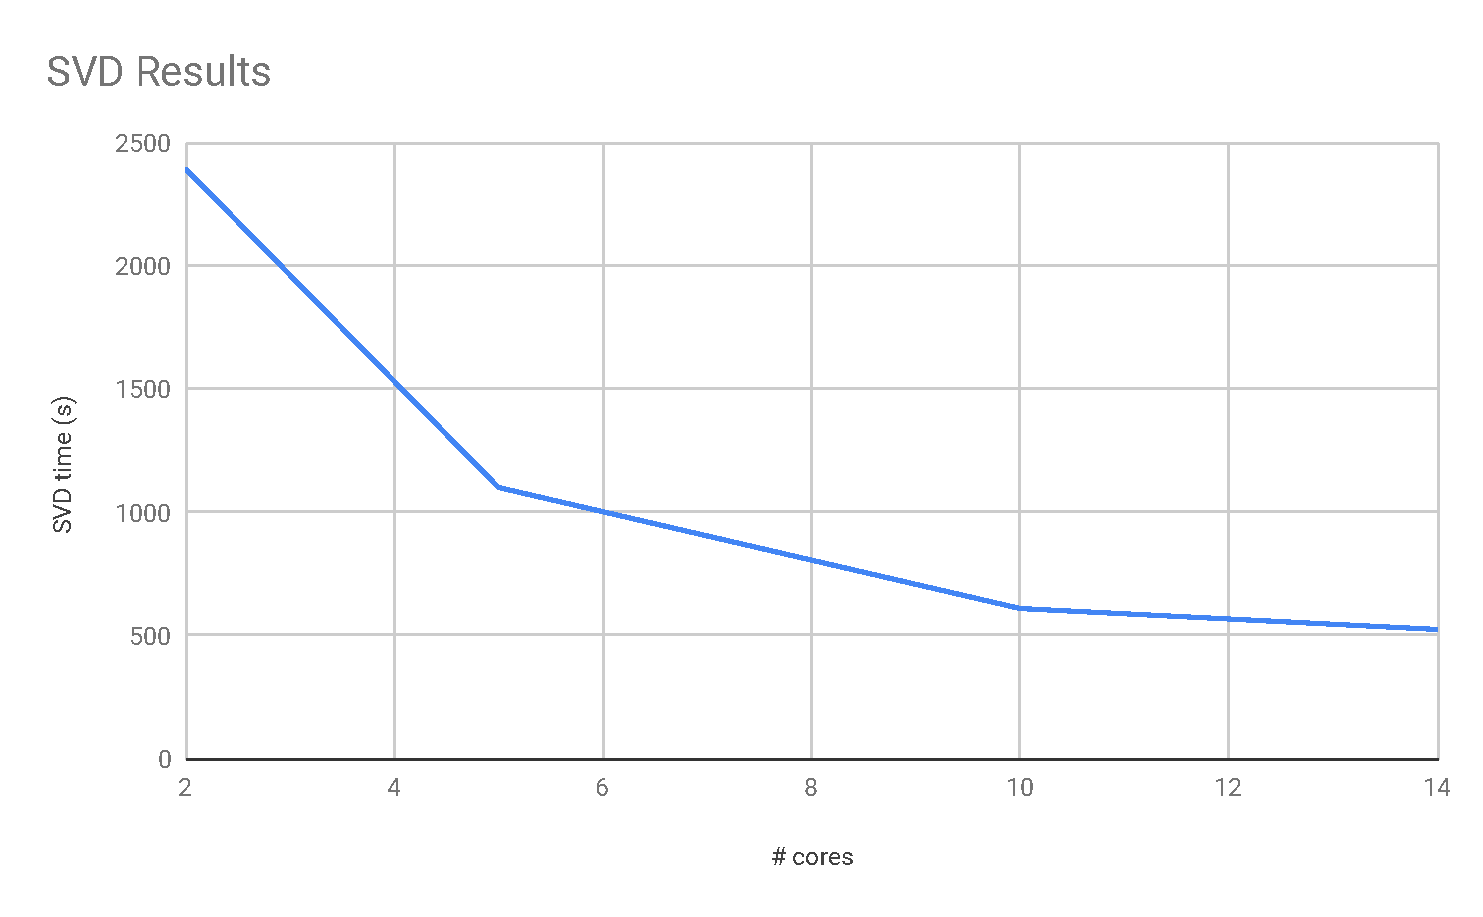
\includegraphics[width=8cm]{SVD Results.pdf}
\end{center}
\caption{The figure show}\label{svd}
\end{figure}

\section{Conclusion}

\end{document}
